
\section{Progettazione architetturale}
\subsection*{Progettazione delle strutture dati}
La prima fase della progettazione architetturale è stata la progettazione delle strutture dati. 
Era molto importante progettare le strutture dati in modo da poterle utilizzare in modo efficiente e 
veloce, in quanto il progetto si basa su di esse.\\
L'obiettivo era quello di creare una struttura dati che permettesse di rappresentare un grafo di dipendenze tra i vari pacchetti di un progetto.
Ogni nodo del grafo rappresenta un pacchetto, ed aveva bisogno delle seguenti informazioni:
\begin{itemize}
  \item \textbf{id}: identificativo univoco del nodo;
  \item \textbf{\textit{group}}: nome del gruppo del pacchetto;
  \item \textbf{\textit{name}}: nome del pacchetto;
  \item \textbf{\textit{version}}: versione del pacchetto;
  \item \textbf{tipo}: tipo del pacchetto, può essere Java o JavaScript;
\end{itemize}

\noindent Ogni arco del grafo, come mostrato in figura \ref*{fig:esempio1-neo4j}, rappresenta una dipendenza tra due pacchetti, 
ed ha bisogno delle seguenti informazioni:
\begin{itemize}
  \item \textbf{id}: identificativo univoco dell'arco;
  \item \textbf{from}: identificativo del nodo di partenza;
  \item \textbf{to}: identificativo del nodo di arrivo;
  \item \textbf{require}: numero di versione richiesto dal pacchetto di partenza;
  \item \textbf{variants}: rappresenta la lista di utilizzi del pacchetto, es: \textit{compileOnly, implementation, testImplementation}; 
\end{itemize}

\begin{figure}[!h] 
  \centering 
  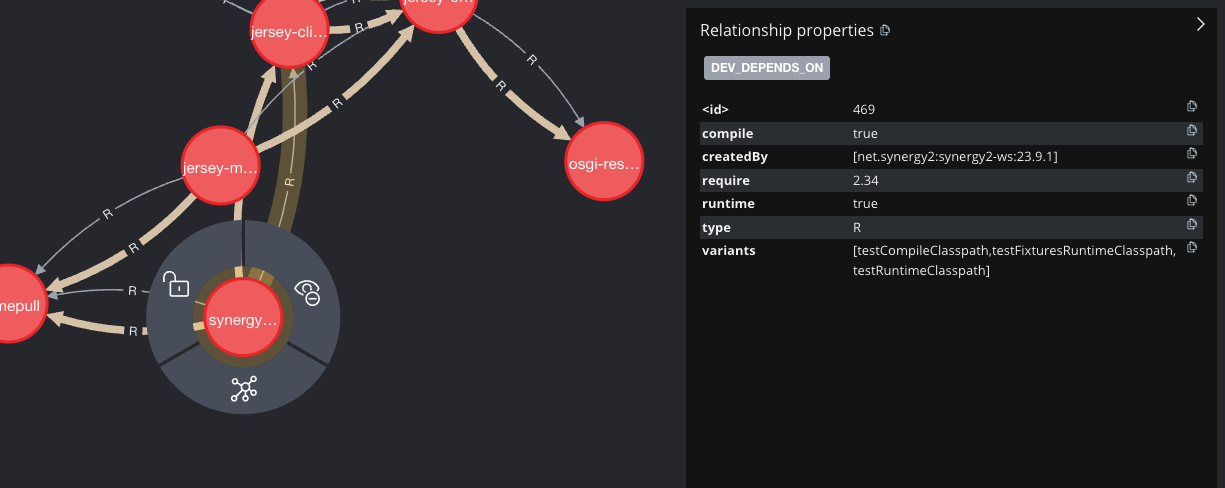
\includegraphics[width=1\columnwidth]{esempio1-neo4j} 
  \caption{Esempio di grafo di dipendenze tra pacchetti.}
  \label{fig:esempio1-neo4j}
\end{figure}

Prima di arrivare alla struttura finale, abbiamo fatto diverse prove, cercando di trovare la struttura più adatta alle nostre esigenze.
La versione finale, come mostrato in figura \ref{fig:struttura-grafo} ha saputo soddisfare tutte le nostre esigenze.\\
Da ogni nodo possono partire tre tipi di archi, ognuno con una funzione diversa.
Il primo tipo di arco è quello che rappresenta 
una dipendenza diretta tra due pacchetti, quindi ad esempio se il pacchetto \textbf{A 1.0} dipende dal pacchetto \textbf{B 1.0}, 
allora dal nodo \textbf{A 1.0} parte un arco, nella figura è rappresentato con una linea continua, che punta al nodo \textbf{B 1.0}.\\
Il secondo tipo di arco è quello che rappresenta una dipendenza transitiva tra due pacchetti, quindi ad esempio se il pacchetto
\textbf{A 1.0} dipende dal pacchetto \textbf{C 1.0} e il pacchetto \textbf{C 1.0} dipende dal pacchetto \textbf{D 3.0},
allora dal nodo A parte un arco, nella figura è rappresentato con una linea tratteggiata, che punta al nodo \textbf{D 3.0}.\\
Il terzo ed ultimo tipo di arco è quello che rappresenta una dipendenza transitiva tra due pacchetti, ma con una versione diversa,
quindi ad esempio se il pacchetto \textbf{A 1.0} dipende dal pacchetto \textbf{B 1.0} e il pacchetto \textbf{B 1.0} dipende dal pacchetto 
\textbf{D 2.0}, ma il pacchetto \textbf{A 1.0} dipende anche, in modo diretto o transitivo, dal pacchetto \textbf{D 3.0}, 
allora dal nodo \textbf{B 1.0} parte un arco, nella figura è rappresentato con una linea tratteggiata, a tratto più piccolo, 
che punta al nodo \textbf{D 3.0}.\\
Questo ultimo tipo di arco l'abbiamo introdotto per poter gestire le dipendenze transitiva con versioni diverse, dato che al rilascio di un
pacchetto finale da installare, la versione che verrà installata sarà quella più recente, in questo caso la versione \textbf{D 3.0}.\\

\begin{figure}[!h] 
  \centering 
  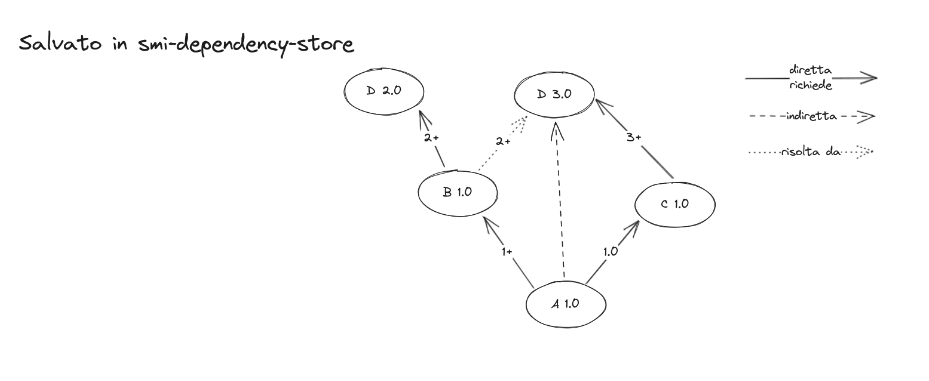
\includegraphics[width=1\columnwidth]{struttura-grafo} 
  \caption{Struttura finale del grafo di dipendenze.}
  \label{fig:struttura-grafo}
\end{figure}

\subsection*{Progettazione \textit{plugin} di analisi delle dipendenze}

Il progetto Java per la creazione del \textit{plugin} Gradle, smi-dependency-analyzer, è stato sviluppato utilizzando il \textit{framework} Gradle.\\
Gradle mette a disposizione delle \textit{API} per la creazione di \textit{plugin} personalizzati,
che permettono di estendere le funzionalità del \textit{build tool}.\\
Il progetto contiene tre \textit{package} principali:
\begin{itemize}
  \item \textbf{\textit{model}}: contiene le classi che rappresentano le strutture dati utilizzate dal \textit{plugin};
  \item \textbf{\textit{logic}}: contiene le classi che rappresentano la logica del \textit{plugin}, dove vengono eseguite le operazioni di analisi, 
  trasformazione e trasferimento dei dati;
  \item \textbf{task}: contiene le classi che rappresentano i \textit{task} del \textit{plugin}, ovvero le operazioni che possono essere eseguite dal \textit{plugin} 
  e la classe di registrazione del \textit{plugin}.
\end{itemize}

Ho definito anche una classe che rappresenta l'oggetto di configurazione del \textit{plugin}, 
che contiene le informazioni necessarie per l'esecuzione del \textit{plugin} e per il salvataggio dei dati, un esempio lo si può visualizzare nel frammento di codice \ref*{lst:plugin-config}

\begin{lstlisting}[
  language=Groovy, 
  caption={Esempio di configurazione del \textit{plugin} Gradle, utilizzando il linguaggio Groovy.},
  captionpos=b, 
  label={lst:plugin-config}
  ]
  smi_dependency_analyzer {
    username = "nome_utente"
    password = "private_key"
    url = "http://localhost:8080/smi-dependency-store"
    npmProject {
        packageJson = "/projects/esempio1/client/package.json"
        packageLockJson = "/projects/esempio1/client/package-lock.json"
    }
  }
\end{lstlisting}

L'idea di base del \textit{plugin} è quella di creare un \textit{task} che avvii il \textit{task standard} messo a disposizione da Gradle
per la creazione del \textit{dependency tree}, ovvero \textit{dependencyInsight}, e con l'\textit{output} di questo \textit{task},
creare un grafo di dipendenze, che verrà inviato al \textit{server} per essere salvato.\\
Per i proggetti Npm invece, il \textit{plugin} legge il file \textit{package-lock.json}. Questo file viene generato automaticamente
da Npm e contiene tutte le informazioni necessarie per la creazione del grafo di dipendenze.
Un prerequisito per il funzionamento del \textit{plugin} è che sia stato eseguito il comando \textbf{\textit{npm install}},
in modo da avere tutte le dipendenze installate nella cartella \textit{node\_modules} e quindi avere il file \textit{package-lock.json}.

Una volta raccolte tutte le informazioni necessarie, effettuo una chiamata \textit{REST} di tipo \textit{PUT} al \textit{server},
per salvare il grafo di dipendenze.\\
\subsection*{Progettazione \textit{backend}}
Il progetto del \textit{backend}, denominato \textbf{smi-dependency-store}, l'ho suddiviso in quattro \textit{package} principali:
\begin{itemize}
  \item \textbf{model}: contiene le classi che rappresentano le strutture dati utilizzate dal \textit{server} e 
  le classi di configurazione;
  \item \textbf{dao}: contiene le classi utilizzate per la comunicazione con il \textit{database}, ed in questo caso
  conteneva la classe \textbf{PackageNodeDao} che gestiva l'inserimento/aggiornamento/cancellazione dell'entità nodo \textbf{PackageNode}
  e la classe \textbf{DependencyLinkDao} che gestiva l'inserimento/aggiornamento/cancellazione dell'entità arco \textbf{DependencyLink};
  \item \textbf{logic}: contiene le classi che rappresentano la logica del \textit{server}, dove vengono eseguite le operazioni di analisi, 
  trasformazione e chiamate alle classi \textit{dao};
  \item \textbf{rest}: contiene le classi che rappresentano i \textit{controller} del \textit{server}, 
  ovvero tutti i servizi \textit{REST} messi a disposizione dal \textit{server}.
\end{itemize}

Per la configurazione del \textit{server}, ho previsto quattro diversi file di configurazione, uno per ogni funzionalità del \textit{server}:
\begin{itemize}
  \item \textbf{neo4j.yml}: contiene le informazioni per la connessione al \textit{database} Neo4j, come l'indirizzo, l'username e la password. Vedi snippet \ref*{lst:neo4j-config};
  \begin{lstlisting}[
    caption={Esempio di configurazione del \textit{neo4j.yml}}
    captionpos=b, 
    label={lst:neo4j-config}
    ]
  url: "bolt://localhost:7689"
  username: "neo4j"
  password: "neo4jlocal"
  \end{lstlisting}
  \item \textbf{token.yml} contiene le informazioni per la generazione del \textit{token}, come la chiave segreta, il \textit{clientId}, il \textit{clientSecret}, il
    nome del \textit{server} e la durata del \textit{token}. Vedi snippet \ref*{lst:token-config}.
    Questo vuol dire che se non configurato l'\textit{LDAP}, ci sarà un solo utente che potrà accedere al \textit{server}, 
    utilizzando come \textit{username} e \textit{password} quelle configurate come \textit{clientId} e \textit{clientSecret}.\\
    Il token \textit{JWT} generato avrà una durata di 30 minuti e sarà firmato con la chiave segreta \textit{SECRET\_KEY}.
    \begin{lstlisting}[caption={Esempio di configurazione del \textit{token.yml}.},captionpos=b, label={lst:token-config}]
  hmacSha512Key: "SECRET_KEY"
  clientId: "admin"
  clientSecret: "admin"
  issuer: "dependency_store"
  validity: 1800000
    \end{lstlisting}
  \item \textbf{logger.yml}: contiene le informazioni per la configurazione del \textit{logger}, come il livello di log, il formato del \textit{log} e il file di output. Vedi snippet \ref*{lst:logger-config}.
    Questa configurazione viene passata ad una libreria sviluppata da \azienda{}, che è un \textit{wrapper} della libreria \textit{slf4j}, nota libreria per la gestione dei \textit{log} in Java.
    Il campo \textit{params} contiene le informazioni per la configurazione del livello di \textit{log} per ogni \textit{package} del \textit{server}, molto utile per la fase di \textit{debug}.
    \begin{lstlisting}[caption={Esempio di configurazione del \textit{logger.yml}.},captionpos=b, label={lst:logger-config}]
defaultLogLevel: "info"
showDateTime: true
dateTimeFormat: "yyyy-MM-dd HH:mm:ss"
showThreadName: false
showShortLogName: true
logFile: "../logs/out.log"
  params:
   com.smi: "debug"
  \end{lstlisting}
 \item \textbf{ldap.yml} contiene le informazioni per la configurazione dell'\textit{LDAP}, come l'indirizzo del \textit{server}, 
 il dominio ed un \textit{flag} che indica se utilizzare una connessione sicura o meno. Vedi snippet \ref*{lst:ldap-config}.
  \begin{lstlisting}[caption={Esempio di configurazione dell'\textit{ldap.yml}.},captionpos=b, label={lst:ldap-config}]
  url: "ldap://10.10.99.1"
  domain: "DOMIONIO_AZIENDA"
  ssl: false
  \end{lstlisting}
\end{itemize}

Per l'implementazione delle classi Java dedicate alla logica, \textit{dao} e di configurazione ho adottato il 
\textit{design pattern} \textit{Singleton}; 
Questo approccio assicura che esista una sola istanza di queste classi 
all'interno del \textit{server}, utilizzata condivisamente da tutte le altre classi.

Per realizzare il \textit{Singleton} in Java, ho sfruttato una libreria sviluppata da \azienda{}, che facilita 
l'implementazione di questo pattern in modo efficiente e rapido. L'\textit{snippet} \ref*{lst:esempio-singleton} mostra un esempio 
di questa implementazione per la classe \textbf{PackageNodeDao}. Abbiamo optato per l'uso di una \textit{inner class} statica, 
dotata di un campo statico \textbf{SingletonHolder}. Quest'ultimo contiene un metodo \textit{get} che accetta una \textit{lambda expression}, 
restituendo un oggetto di tipo \textbf{PackageNodeDao}. Questa strategia garantisce la creazione dell'istanza solo all'occorrenza, 
evitando la creazione anticipata al momento del caricamento della classe e assicurando l'unicità dell'istanza anche in contesti di \textit{multithreading}.

La classe \textbf{SingletonHolder} non solo gestisce la creazione dell'istanza, ma offre anche la possibilità di personalizzare i metodi 
di \textbf{PackageNodeDao}. Se si desidera modificare i metodi di questa classe, è possibile definire una sottoclasse di \textbf{PackageNodeDao}, 
nominata \textbf{PackageNodeDaoPers}. In questo caso, grazie all'uso della \gls{reflection} di Java, 
il \textbf{SingletonHolder} restituirà automaticamente un'istanza di \textbf{PackageNodeDaoPers}, permettendo una personalizzazione avanzata.
\newpage


\begin{lstlisting}[
  language=Java, 
  caption={Esempio di implementazione del \textit{design pattern} Singleton in Java.},
  captionpos=b, 
  label={lst:esempio-singleton}
  ]
  public class PackageNodeDao {
    protected PackageNodeDao () { }
    public static PackageNodeDao get() {
      return Singleton.INSTANCE.get(PackageNodeDao::new);
    }
    private static class Singleton {
        private static final SingletonHolder<PackageNodeDao> INSTANCE = new SingletonHolder<> (PackageNodeDao.class);
    }
  }
\end{lstlisting}

\subsection*{Progettazione \textit{frontend}}

Per la progettazione del \textit{frontend} ho seguito il \textit{mockup} grafico realizzato in fase di analisi.\\
Questo ci ha permesso di avere una visione chiara e dettagliata dell'interfaccia grafica, 
semplificando notevolmente la fase di sviluppo.\\
Il \textit{mockup} è stato realizzato utilizzando il \textit{tool} gratuito \textit{online} \textit{excalidraw}, che permette di creare grafiche semplici
come quella mostrata in figura \ref*{fig:mockup}.\\
\begin{figure}[!h] 
  \centering 
  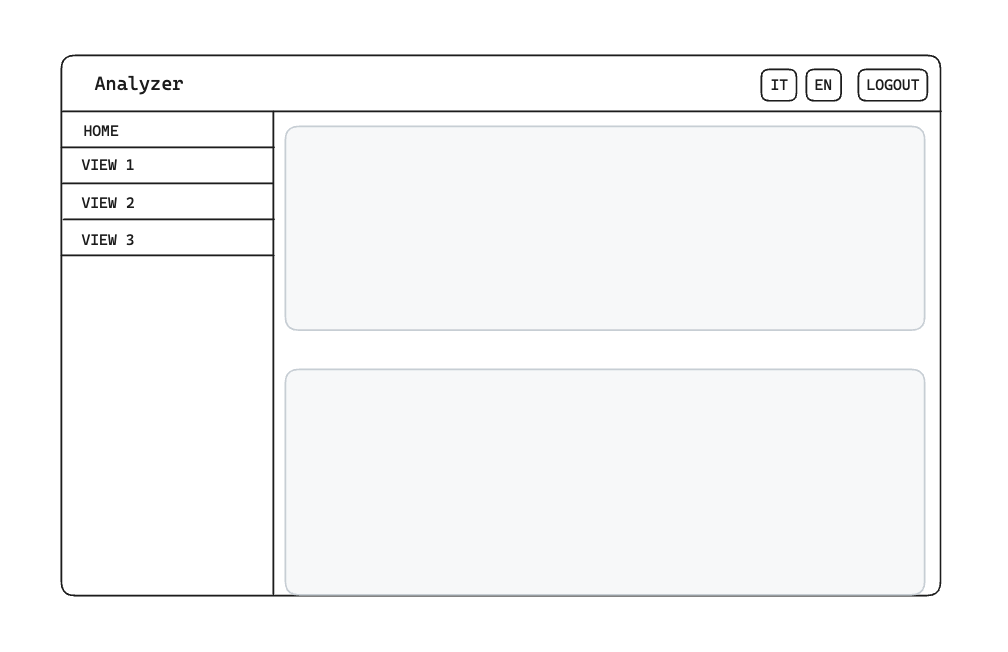
\includegraphics[width=1\columnwidth]{mockup} 
  \caption{\textit{Mockup} grafico dell'interfaccia grafica.}
  \label{fig:mockup}
\end{figure}

Da qui ho iniziato a sviluppare il \textit{frontend}, utilizzando il \textit{framework} Angular.\\
Per prima cosa creato le due cartelle principali del progetto, la prima, \textbf{commons}, contiene i componenti, i servizi e i modelli che possono 
essere utilizzati in più componenti;
la seconda, \textbf{features}, contiene a sua volta una cartella per ogni funzionalità del \textit{frontend}.
Ho creato quindi le cartelle \textbf{home}, \textbf{login}, \textbf{query} e \textbf{find-by-project}. 
  Ogni cartella al suo interno contiene i componenti, i servizi e i modelli relativi alla funzionalità. 
  Nella figura \ref*{fig:frontend-structure} è possibile vedere la struttura del progetto.
  \begin{figure}[!h] 
    \centering
    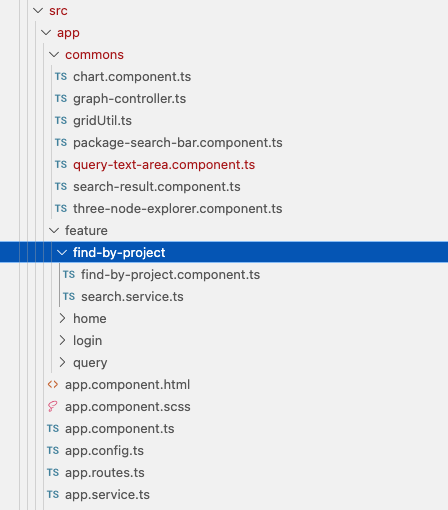
\includegraphics[width=.5\columnwidth]{frontend-structure} 
    \caption{Struttura del progetto \textit{frontend}.}
    \label{fig:frontend-structure}
  \end{figure}  

Per la scrittura del codice ho seguito le linee guida di Angular, rilasciate nel loro sito ufficiale \cite{site:angular-style-guide}.\\

Come mostrato in figura \ref*{fig:frontend-1}, l'interfaccia grafica è formata da una barra di navigazione, che contiene il nome del progetto,
il pulsante per il \textit{logout} ed i pulsanti per cambiare la lingua dell'interfaccia grafica.\\
Sotto la barra di navigazione è presente una \textit{sidebar}, che contiene i pulsanti per accedere alle varie funzionalità del \textit{frontend} 
ed il contenitore principale che mostra il contenuto della funzionalità selezionata.\\
\begin{figure}[!h]
  \centering
  \begin{minipage}{0.45\textwidth}
      \centering
      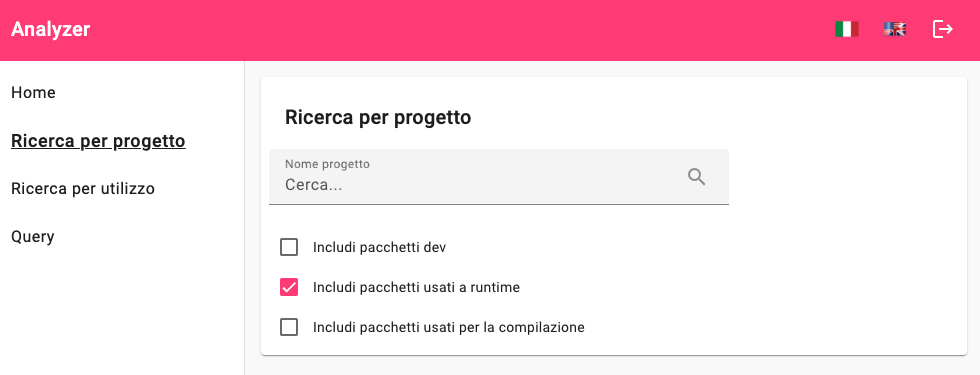
\includegraphics[width=\textwidth]{frontend-1}
      \caption{Modulo di ricerca dipendenze per progetto.}
      \label{fig:frontend-1}
  \end{minipage}\hfill
  \begin{minipage}{0.45\textwidth}
      \centering
      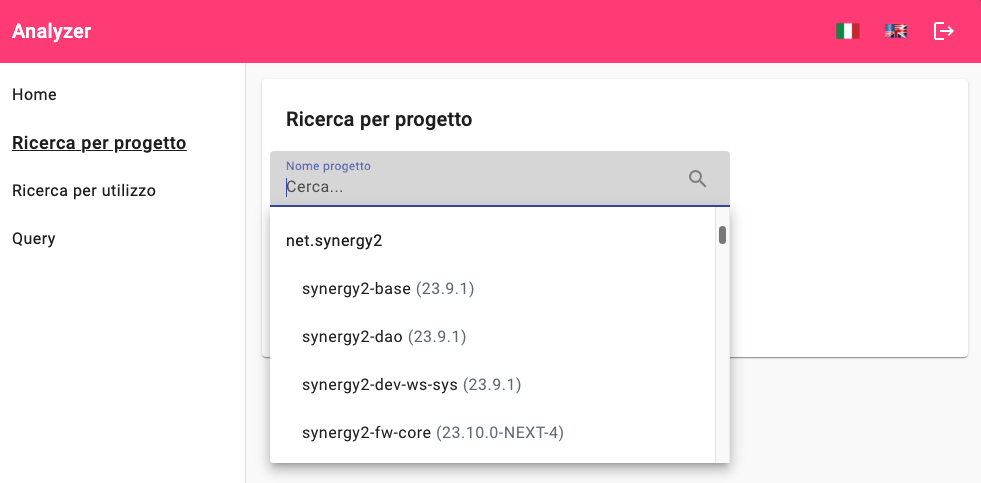
\includegraphics[width=\textwidth]{frontend-2}
      \caption{Casella di ricerca con lista di suggerimenti.}
      \label{fig:frontend-2}
  \end{minipage}
\end{figure}
Le voci di menu presenti nella \textit{sidebar}, oltre alla funzionalità \textit{home}, sono tre:
\begin{itemize}
  \item \textbf{Ricerca per progetto}: Come mostrato in figura \ref*{fig:frontend-1}, in questo modulo, tramite la barra di ricerca
   è possibile inserire il nome completo, formato da \textit{group}, \textit{name} e \textit{version}, di un pacchetto e visualizzare
    le informazioni relative a quel pacchetto.\\
    Tuttavia per rendere più semplice la ricerca, ho aggiunto una funzionalità di suggerimento, che mostra la lista di pacchetti conosciuti dal 
    \textit{server}, che iniziano con la stringa inserita nella barra di ricerca, mostrandoli raggruppati per \textit{group}, come rappresentato in figura \ref*{fig:frontend-2}.\\
    Sotto la casella di testo sono presenti tre \textit{checkbox}, che permette di scegliere se includere i pacchetti targati come \textit{dev}, 
    se includere i pacchetti utilizzati solo durante la compilazione dei progetti e se includere tutti i pacchetti utilizzati a runtime
    da un progetto.\\
    Una volta avviata la ricerca, viene mostrato il risultato sotto di esso, come mostrato in figura \ref*{fig:frontend-3}.\\
    Qui troviamo tre possibili visualizzazioni del risultato: a grafo, ad albero e a lista.\\
    Nella visualizzazione tabellare abbiamo una lista piatta di tutti i pacchetti, con le informazioni principali, trascurando i collegamenti tra i pacchetti.\\
    Questa visualizzazione può tornare utile quando si vuole avere una visione d'insieme di tutti i pacchetti utilizzati da un progetto.\\
    Nella visualizzazione ad albero invece, abbiamo una visualizzazione gerarchica dei pacchetti, dove ogni nodo rappresenta un pacchetto ed espanendo un nodo
    è possibile vedere i pacchetti da cui dipende.\\
    In questo modo riusciamo a capire come mai un pacchetto è stato incluso nel progetto, e quali altri pacchetti sono stati inclusi a causa di esso.\\
    Nella visualizzazione a grafo invece, abbiamo una visualizzazione grafica dei pacchetti, dove ogni nodo rappresenta un pacchetto e gli archi rappresentano
    le dipendenze tra i pacchetti.\\
    \begin{figure}[h]
      \centering
      \begin{minipage}{0.60\textwidth}
          \centering
          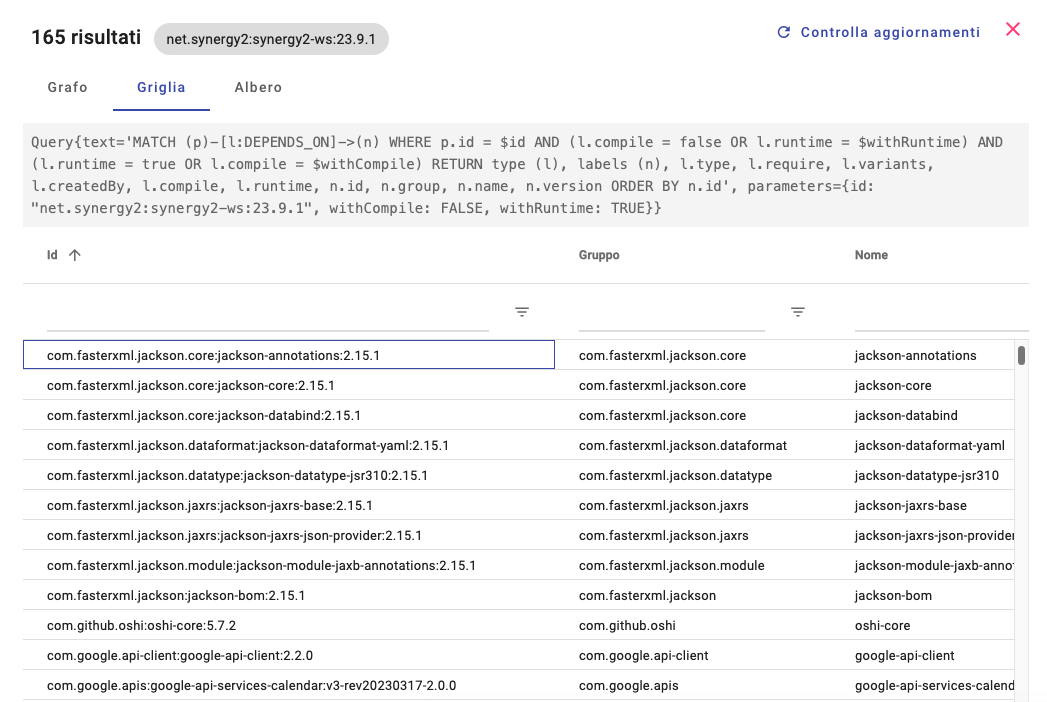
\includegraphics[width=\textwidth]{frontend-3.png} 
          \caption{Risultato tabellare.}
          \label{fig:frontend-3}
      \end{minipage}\hfill
      \begin{minipage}{0.30\textwidth}
          \centering
          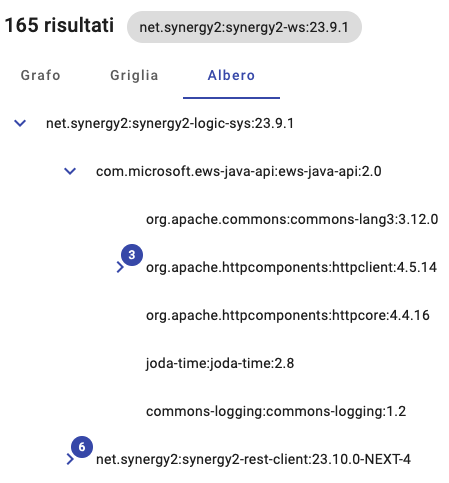
\includegraphics[width=\textwidth]{frontend-4.png} 
          \caption{Risultato ad albero.}
          \label{fig:frontend-4}
      \end{minipage}
    \end{figure}
    Inoltre, è possibile fare un controllo sulla presenza di aggiornamenti e vulnerabilità, ad esempio, come mostrato in figura \ref*{fig:frontend-8},
    vengono mostrati tutti i pacchetti che hanno una versione più recente di quella utilizzata dal progetto.\\
    \begin{figure}[!h] 
      \centering
      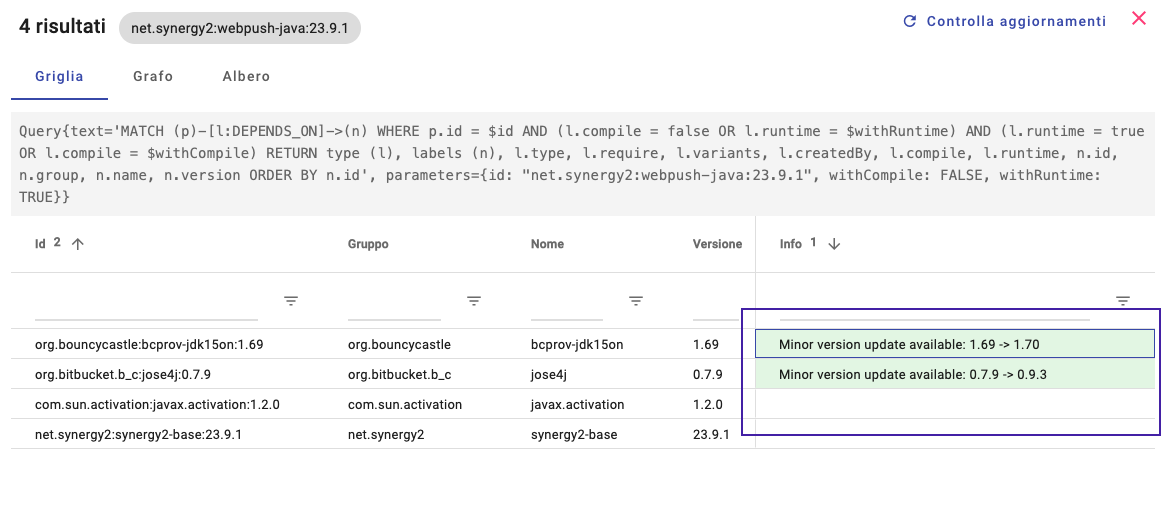
\includegraphics[width=1\columnwidth]{frontend-88.png} 
      \caption{Visualizzazione di tutti gli aggiornamenti disponibili.}
      \label{fig:frontend-8}
    \end{figure}  
  \item \textbf{Ricerca per utilizzo}: La ricerca avviene in modo simile a quella per progetto, ma in questo caso, il risultato mostra solo una 
  griglia con i pacchetti che utilizzano il pacchetto cercato.\\
  Nell'esempio in figura \ref*{fig:frontend-5}, ho cercato il pacchetto \textbf{net.synergy2:synergy2-base:23.9.1}, e il risultato mostra tutti i pacchetti che lo utilizzano.\\
  Oltre alla griglia, è presente anche un \textit{box} che mostra la \textit{query}, con la sintassi Cypher, utilizzata per la ricerca.\\


  \begin{figure}[!h] 
    \centering
    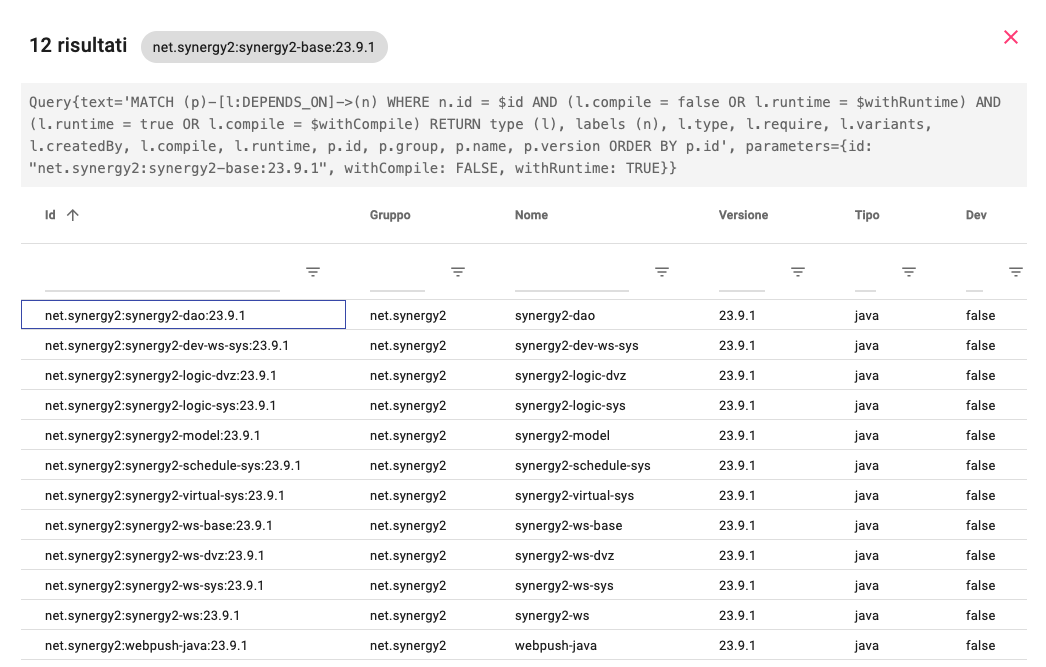
\includegraphics[width=.9\columnwidth]{frontend-5.png} 
    \caption{Esempio di ricerca per utilizzo.}
    \label{fig:frontend-5}
  \end{figure}  
  \item \textbf{\textit{Query}}: in quest'ultima funzionalità, come mostrato in figura \ref*{fig:frontend-5}, è possibile inserire una \textit{query} Cypher libera e visualizzare il risultato in 
  formato \textit{JSON}. Questo può tornare utile quando si vuole effettuare una ricerca più complessa, che non è possibile effettuare con le altre funzionalità.\\
  \begin{figure}[!h] 
    \centering
    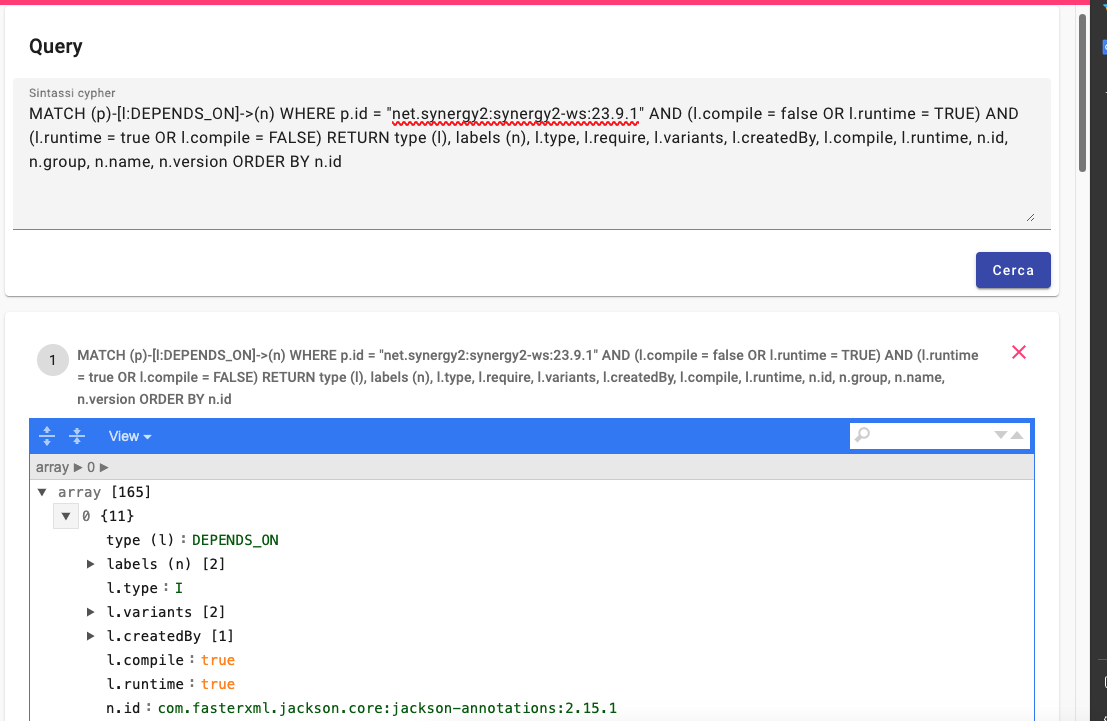
\includegraphics[width=.9\columnwidth]{frontend-6.png} 
    \caption{Modalità \textit{query} libera.}
    \label{fig:frontend-6}
  \end{figure}  

\end{itemize}
